\documentclass[11pt]{article}
\title{\textbf{Statistics Group Assignment}}
\author{Daniel Alkurdi \\ \and Sammi Guan \\ \and Stephanie Yang \\ \and Veda Rena \\ \and William Huynh}
\date{\small{Business Statistics 26134}}

\usepackage[linewidth=0.5pt]{mdframed}
\usepackage{mathtools}

\usepackage{pdfpages}
\usepackage[dvipsnames]{xcolor}
\definecolor{mygray}{gray}{0.9}
\mdfsetup{frametitlealignment=\center}

\usepackage{fancyhdr}

\pagestyle{fancy}
\fancyhf{}
\rhead{\scriptsize Business Statistics 26134}
\lhead{\small \textbf{Group Assignment}}
\cfoot{\thepage} 

\usepackage{subfig}
\usepackage{booktabs}
\usepackage{xcolor}
\usepackage{adjustbox}
\usepackage{csvsimple}
\begin{filecontents*}{counts.csv}
a,online,store
Less than 10 hours,53,44
Between 10 and 20 hours,50,64
More than 20 hours,64,224


\end{filecontents*}
\begin{filecontents}{scattera.csv}
x,y
1,11
2,15
3,10
4,12
5,8
6,17
7,11
8,11
9,13
10,14
11,10
12,14
13,15
14,16
15,6
16,12
17,9
18,6
19,7
20,11
21,13
22,17
23,9
24,15
25,14
26,20
27,11
28,17
29,16
30,8
31,19
32,11
33,6
34,11
35,9
36,8
37,12
38,17
39,12
40,10
41,13
42,19
43,15
44,8
45,12
46,8
47,13
48,14
49,12
50,7
51,11
52,13
53,11
54,17
55,12
56,13
57,9
58,13
59,15
60,16
61,15
62,9
63,13
64,13
65,14
66,15
67,12
68,12
69,8
70,9
71,9
72,9
73,14
74,18
75,10
76,5
77,16
78,16
79,14
80,16
81,9
82,12
83,4
84,6
85,14
86,18
87,5
88,9
89,7
90,8
91,11
92,17
93,7
94,11
95,6
96,12
97,13
98,10
99,19
100,8
101,12
102,8
103,11
104,15
105,19
106,13
107,9
108,13
109,19
110,9
111,6
112,14
113,6
114,12
115,9
116,12
117,10
118,14
119,9
120,8
121,8
122,16
123,10
124,9
125,10
126,7
127,10
128,10
129,14
130,12
131,14
132,13
133,11
134,11
135,17
136,17
137,12
138,14
139,16
140,12
141,9
142,11
143,20
144,5
145,13
146,13
147,12
148,12
149,10
150,9
151,14
152,14
153,12
154,10
155,19
156,7
157,13
158,14
159,10
160,15
161,11
162,11
163,12
164,19
165,11
166,9
167,11
168,15
169,7
170,10
171,10
172,14
173,13
174,12
175,13
176,16
177,9
178,9
179,10
180,10
181,20
182,8
183,8
184,13
185,12
186,19
187,7
188,5
189,15
190,13
191,12
192,14
193,8
194,8
195,14
196,18
197,14
198,8
199,10
200,20
\end{filecontents}
\begin{filecontents}{scatterb.csv}
x,y
1,10
2,9
3,11
4,7
5,8
6,15
7,6
8,8
9,10
10,18
11,11
12,17
13,9
14,17
15,18
16,13
17,4
18,13
19,9
20,14
21,17
22,7
23,17
24,11
25,12
26,17
27,7
28,5
29,15
30,11
31,18
32,10
33,15
34,12
35,12
36,10
37,12
38,17
39,9
40,16
41,17
42,16
43,8
44,17
45,18
46,17
47,11
48,18
49,12
50,11
51,12
52,10
53,11
54,14
55,14
56,9
57,1
58,16
59,6
60,9
61,13
62,8
63,18
64,8
65,18
66,8
67,20
68,10
69,21
70,11
71,10
72,11
73,15
74,15
75,12
76,12
77,14
78,13
79,9
80,1
81,9
82,12
83,17
84,13
85,16
86,6
87,9
88,7
89,17
90,14
91,10
92,18
93,12
94,12
95,13
96,9
97,9
98,8
99,6
100,13
101,14
102,14
103,9
104,15
105,13
106,13
107,10
108,15
109,1
110,15
111,14
112,14
113,21
114,12
115,12
116,10
117,10
118,6
119,5
120,11
121,14
122,8
123,15
124,12
125,14
126,13
127,15
128,14
129,12
130,14
131,9
132,16
133,10
134,16
135,3
136,12
137,11
138,16
139,6
140,10
141,12
142,10
143,14
144,17
145,12
146,20
147,7
148,17
149,14
150,4
151,10
152,14
153,14
154,13
155,10
156,16
157,13
158,11
159,11
160,17
161,8
162,21
163,17
164,14
165,10
166,13
167,18
168,8
169,10
170,16
171,13
172,18
173,9
174,14
175,12
176,8
177,5
178,12
179,10
180,16
181,8
182,15
183,4
184,6
185,5
186,15
187,10
188,18
189,4
190,17
191,10
192,8
193,12
194,17
195,14
196,10
197,20
198,10
199,9
200,9

\end{filecontents}
\usepackage{pgfplots}
\usepackage{pgfplotstable}
\pgfplotstableread[col sep=comma]{counts.csv}\datatable
\makeatletter
\pgfplotsset{
    /pgfplots/flexible xticklabels from table/.code n args={3}{%
        \pgfplotstableread[#3]{#1}\coordinate@table
        \pgfplotstablegetcolumn{#2}\of{\coordinate@table}\to\pgfplots@xticklabels
        \let\pgfplots@xticklabel=\pgfplots@user@ticklabel@list@x
    }
}
\makeatother

\begin{document}

\maketitle

\hrule
\tableofcontents

\newpage
\section{Everstain Investment Group}
\subsection{Frequency Distribution of Monthly Payments for all Employees}

\begin{tabular}{l|cc}
  bin& Frequency& \\
  \hline
  (0, 1000]& 4& \\
  (1000, 2000]& 15&\\
  (2000, 3000]& 42&\\
  (3000, 4000]& 490&\\
  (4000, 5000]& 258&\\
  (5000, 6000]& 109&\\
  (6000, 7000]& 59&\\
  (7000, 8000]& 19&\\
  (8000, 9000]& 3&\\
\end{tabular}
\begin{tikzpicture}[baseline=(current bounding box.east)]
\begin{axis}[
    ybar,
    ymin=0
]
\addplot +[
    hist={
        bins=9,
    }   
] table [y index=0] {all.csv};

\end{axis}

\end{tikzpicture}



\subsection{Frequency Distribution of Monthly Payment of Males}
\begin{tabular}{l|cc}
  bin& Frequency& \\
  \hline
  (0, 1000]& 4& \\
  (1000, 2000]& 15&\\
  (2000, 3000]& 42&\\
  (3000, 4000]& 123&\\
  (4000, 5000]& 118&\\
  (5000, 6000]& 109&\\
  (6000, 7000]& 59&\\
  (7000, 8000]& 18&\\
  (8000, 9000]& 3&\\
  
\end{tabular}
\begin{tikzpicture}[baseline=(current bounding box.east)]
\begin{axis}[
    ybar,
    ymin=0,
    xmin=0,
    xmax=9000,
    ymax=600,
]
\addplot +[
    hist={
        bins=9,
    }   
] table [y index=0] {males.csv};

\end{axis}

\end{tikzpicture}
\newpage

\subsection{Frequency Distribution of Monthly Payment of Females}
\begin{tabular}{l|cc}
  bin& Frequency& \\
  \hline
  (0, 1000]& 0& \\
  (1000, 2000]& 0&\\
  (2000, 3000]& 0&\\
  (3000, 4000]& 367&\\
  (4000, 5000]& 140&\\
  (5000, 6000]& 0&\\
  (6000, 7000]& 0&\\
  (7000, 8000]& 0&\\
  (8000, 9000]& 0&\\
  
\end{tabular}
\begin{tikzpicture}[baseline=(current bounding box.east)]
\begin{axis}[
    ybar,
    ymin=0,
    xmin=0,
    xmax=9000,
    ymax=600,
]
\addplot +[
    hist={
        bins=9,
    }   
] table [y index=0] {females.csv};

\end{axis}

\end{tikzpicture}

\subsection{Descriptive Statistics Summary}
The population is defined as the total number of employees in the company, with the subsets of the population (Gender: Male and Female) being samples A and B respectively.
\begin{table}[h]
\centering
\begin{tabular}{@{}lclll@{}}
\toprule
\multicolumn{5}{c}{\textbf{Company (\$) (N=1000)}}              \\ \midrule
Mean $\mu$          & \multicolumn{4}{c}{4244.59}    \\
Median $\widetilde{x}$          & \multicolumn{4}{c}{3975.79}    \\
Variance $\sigma^2$             & \multicolumn{4}{c}{1135892.69} \\
Standard Deviation $\sigma$   & \multicolumn{4}{c}{1065.78}    \\ \bottomrule
\end{tabular}
\end{table}
\begin{table}[h]
\begin{tabular}{@{}lclll@{}}
\toprule
\multicolumn{5}{c}{\textbf{Male (\$) (n=492)}}              \\ \midrule
Mean $\bar{x}_A$          & \multicolumn{4}{c}{4565.70}    \\
Variance $s_A^2$             & \multicolumn{4}{c}{2089960} \\
Standard Deviation $s_A$   & \multicolumn{4}{c}{1445.67}    \\ \bottomrule
\end{tabular}
\begin{tabular}{@{}lclll@{}}
\toprule
\multicolumn{5}{c}{\textbf{Female (\$) (n=508)}}              \\ \midrule
Mean $\bar{x}_B$          & \multicolumn{4}{c}{3933.59}    \\
Variance $s_B^2$             & \multicolumn{4}{c}{19440} \\
Standard Deviation $s_B$   & \multicolumn{4}{c}{139.43}    \\ \bottomrule
\end{tabular}
\end{table}

\newpage \subsection{Gender Pay Gap Calculation}

The Australian Workplace Gender Equality Agency (WGEA) provides information on calculating the gender pay gap.\footnote{Cassells, R., Duncan, A.S. and Ong, R., 2017. Gender equity insights 2017: Inside Australia’s gender pay gap (No. GE02). Bankwest Curtin Economics Centre (BCEC), Curtin Business School.}

\begin{mdframed}[
frametitle={Gender Pay Gap},
frametitlerule=true,
frametitlebackgroundcolor=mygray
]
\begin{center}
\begin{equation}
GPG = 100 \times \dfrac{\bar{x}_A-\bar{x}_B}{\bar{x}_A}	
\end{equation}
\hspace{1cm}
\begin{equation}
	GPG = 100 \times \dfrac{4565.70-3933.59}{4565.70}	
\end{equation}
\hspace{1cm}
\begin{equation}
	GPG = 13.84\%
\end{equation}
\end{center}
\hspace{1cm}
\end{mdframed}

The Gender Pay Gap (GPG) is expressed as a percentage of male earnings. The above results show a 13.84\% difference in the monthly salary of males and females. This GPG calculation is non-adjusted, meaning specific job functions of employees are not considered.

\subsection{Summary of findings}
There is a difference in monthly wages between males and females within Everstain Investment Group. All females within the company earn between \$3000 and \$5000. While male salaries are more normally distributed. Noting there is an approximately 14\% difference in male and female salaries, it is important to note that job functions are not considered in these results. We advise Everstain Investment Group to collect more data in order to compare gender wages within job categories. Two possibilities exist with job functions considered:
\begin{enumerate}
	\item Females are paid less than males
	\item Males tend to have more job functions within the company
\end{enumerate}

Understanding which of the two scenarios is occurring may help Everstain Investment Group to improve reducing their gender pay gap.
\newpage
\section{Warhammer}
\subsection{Contingency Tables}
\subsubsection{Counts}


\begin{table}[hbt]
\centering
\begin{adjustbox}{max width=\columnwidth}
\begin{tabular}{@{}lllll@{}}
\toprule
\multicolumn{5}{c}{\textbf{Contingency Table: Count}}                                                                                  \\ \midrule
                  & Time \textless 10 Hours & 10 Hours \textless Time \textless 20 Hours & Time \textgreater 20 Hours & \textbf{Total} \\
Online Shopping   & 53                      & 50                                         & 64                         & 167            \\
In-Store Shopping & 44                      & 64                                         & 224                        & 333            \\
\textbf{Total}    & 97                      & 115                                        & 288                        & 500            \\ \bottomrule
\end{tabular}
\end{adjustbox}
\end{table}

\subsubsection{Relative Frequency}

\begin{table}[hbt]
\centering
\begin{adjustbox}{max width=\columnwidth}
\begin{tabular}{@{}lllll@{}}
\toprule
\multicolumn{5}{c}{\textbf{Contingency Table: Relative Frequency}}                                                                     \\ \midrule
                  & Time \textless  10 Hours & 10 Hours \textless Time \textless 20 Hours & Time \textgreater 20 Hous & \textbf{Total} \\
Online Shopping   & 0.106                    & 0.100                                      & 0.128                     & 0.334          \\
In-Store Shopping & 0.088                    & 0.128                                      & 0.448                     & 0.664          \\
\textbf{Total}    & 0.194                    & 0.228                                      & 0.576                     & 1              \\ \bottomrule
\end{tabular}
\end{adjustbox}
\end{table}

\subsection{Graphs}

\begin{tikzpicture}
\begin{axis} [
title=\textbf{Time spent with friends and shopping preference},
width=13cm,
height=7cm,
grid=major,
legend pos=outer north east,
ylabel=Number of people,
flexible xticklabels from table={counts.csv}{a}{col sep=comma},
xticklabel style={text height=1.5ex}, % To make sure the text labels are nicely aligned
xtick=data,
nodes near coords,
every node near coord/.append style={anchor=south east,
    inner ysep=0.5pt}]

\addplot table[x expr=\coordindex,y=online]{\datatable};
\addlegendentry{On-line}
\addplot table[x expr=\coordindex,y=store]{\datatable};
\addlegendentry{In-store}
\end{axis}
\end{tikzpicture}

\begin{center}
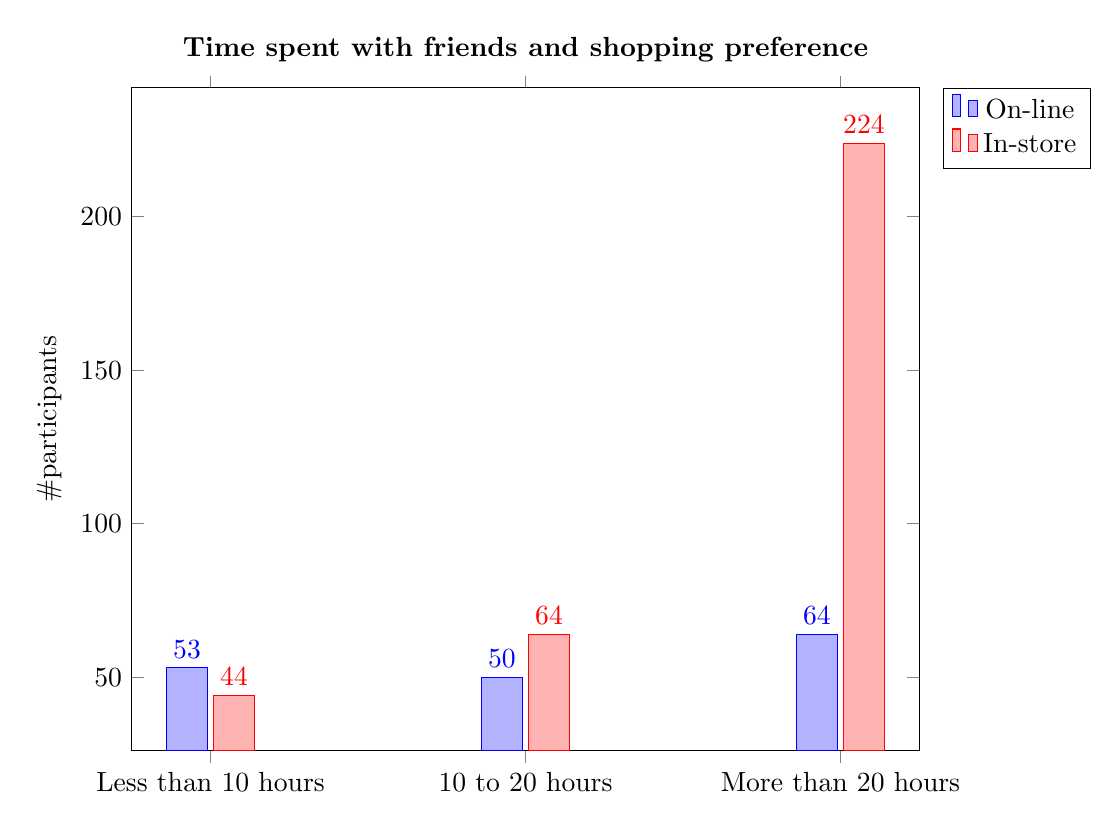
\begin{tikzpicture}
\begin{axis}[
	title=\textbf{Time spent with friends and shopping preference},
	width=6cm,
	height=10cm,
    ybar,
    x=4cm,
    enlarge x limits={abs=1cm}, % The distance between the center of the first bar and the left edge
    bar width=15pt,
  legend pos=outer north east,
    ylabel={\#participants},
    symbolic x coords={Less than 10 hours,10 to 20 hours,More than 20 hours},
    xtick=data,
    nodes near coords,
    nodes near coords align={vertical},
    ]
\addplot coordinates {(Less than 10 hours,53) (10 to 20 hours,50)(More than 20 hours,64) };
\addplot coordinates {(Less than 10 hours,44) (10 to 20 hours,64)(More than 20 hours,224) };
\legend{On-line,In-store,}
\end{axis}
\end{tikzpicture}
\end{center}

\subsection{Is time spent with friends and shopping behaviour independent?}

The procured results suggest that as people spend more time with their friends they tend to spend more time shopping In-store. This correlates with the assumption that people enjoy participating in activities with their friends. Intuitively, the results suggest that time spent with friends and their shopping behaviour may not be independent. Further statistical analysis (correlation tests) may provide Warhammer with a better suggestion as to whether these two variables are independent.
\newpage
\subsection{Summary}

From the analysis we have provided, we believe there is a positive relationship between the time that people spend with their friends and the propensity to;

\begin{enumerate}
\item Partake in shopping activity
\item Shop in-store rather than on-line
\end{enumerate}

As such, we suggest to Warhammer to consider placing more weight towards off-line marketing such as in-store advertisements. However, it is important to note that there is a proportion of customers who do undertake their shopping on-line. Furthermore, with the virtually global use of the internet, on-line advertising is an important factor in the marketing of the brand. A study has found that on-line advertising has shown to have a positive impact on buyers' purchase decision. However, it notes that heterogeneous advertising has the most beneficial impact on a firm's economic activity.\footnote{Bayer, E., Srinivasan, S., Riedl, E.J. and Skiera, B., 2020. The impact of online display advertising and paid search advertising relative to offline advertising on firm performance and firm value. International Journal of Research in Marketing.}

\newpage\section{Istanbul International Airport}
\subsection{Data}
\subsubsection{Visualisation}
\begin{figure}[h!]
\centering 
\begin{tikzpicture}
    \begin{axis}[
    	title=\textbf{Carousel A},
    	scale=0.7,
        xlabel=Minutes, % label x axis
        ylabel=Number of Baggages, % label y axis
        axis lines=left, %set the position of the axes
        clip=false
    ]

            \addplot[scatter, only marks] table [x=x, y=y, col sep=comma] {scattera.csv};
            \addplot[thin, red] table [col sep = comma,y={create col/linear regression={y=y}}]{scattera.csv};

    \end{axis}

\end{tikzpicture}\begin{tikzpicture}
    \begin{axis}[
    	title=\textbf{Carousel B},
    	scale=0.7,
        xlabel=Minutes, % label x axis
        ylabel=Number of Baggages, % label y axis
        axis lines=left, %set the position of the axes
        clip=false
    ]

            \addplot[scatter, only marks] table [x=x, y=y, col sep=comma] {scatterb.csv};
            \addplot[thin, red] table [col sep = comma,y={create col/linear regression={y=y}}]{scatterb.csv};

    \end{axis}

\end{tikzpicture}\end{figure}
\subsubsection{Descriptive Statistics Summary}
% Please add the following required packages to your document preamble:
% \usepackage{booktabs}
\begin{table}[h]
\centering
\begin{tabular}{@{}lll@{}}
\toprule
\multicolumn{3}{l}{\textbf{Carousel A ($n$=200)}}         \\ \midrule
Mean $\bar{x}_a$                       & \multicolumn{2}{l}{11.89}  \\
Median                     & \multicolumn{2}{l}{12}     \\
Mode                       & \multicolumn{2}{l}{12}     \\
Standard Deviation         & \multicolumn{2}{l}{3.57}   \\
Sample Variance            & \multicolumn{2}{l}{12.74}  \\
Kurtosis                   & \multicolumn{2}{l}{-0.411} \\
Skewness                   & \multicolumn{2}{l}{0.246}  \\
Range                      & \multicolumn{2}{l}{16}     \\ \bottomrule
\end{tabular}
\qquad
\begin{tabular}{@{}lll@{}}
\toprule
\multicolumn{3}{l}{\textbf{Carousel B ($n$=200)}}         \\ \midrule
Mean $\bar{x}_b$                      & \multicolumn{2}{l}{12.02}  \\
Median                     & \multicolumn{2}{l}{12}     \\
Mode                       & \multicolumn{2}{l}{10}     \\
Standard Deviation         & \multicolumn{2}{l}{4.10}   \\
Sample Variance            & \multicolumn{2}{l}{16.82}  \\
Kurtosis                   & \multicolumn{2}{l}{-0.217} \\
Skewness                   & \multicolumn{2}{l}{-0.190} \\
Range                      & \multicolumn{2}{l}{20}     \\ \bottomrule
\end{tabular}
\end{table}
From the above results, we can see that the mean of Carousel B is marginally higher than that of Carousel A. Furthermore the number of bags that go through Carousel B have a higher variance than that of Carousel A. 
\newpage
\subsection{Computations}
\subsubsection{Average time to wait to see the next bag}

If we assume that the time which elapses between two events  follows the exponential distribution with a mean of $\mu$ units of time. Additionally assuming that these times are independent, meaning that the time between events is not affected by the times between previous events. If these assumptions hold, then the number of events per unit time follows a Poisson distribution with mean $\lambda = 1/\mu$.

\begin{mdframed}
\begin{center}
\begin{equation}
E(X)=\frac{1}{\lambda}
\end{equation}
\hspace{1cm}
\begin{equation}
E(X)=\frac{1}{11.89}=0.0833
\end{equation}
\hspace{1cm}
\begin{equation}
0.0833 \times 60 = 5
\end{equation}
\hspace{1cm}
\end{center}
\hspace{1cm}
\end{mdframed}
These calculations show that it will take on average, 5 seconds for the next bag to arrive in each Carousel.
\subsubsection{Probability Calculations}
 Probability that there are less than 7 bags in one minute.\\
Let $x$ be the number of bags collected per minute. With $\lambda$ being 12
\begin{mdframed}
\begin{center}
\begin{equation}
P(X=x;\lambda)=\frac{\lambda^x e^{-\lambda}}{x!}
\end{equation}
\hspace{1cm}
\begin{equation}
P(X\leq6;12)=\frac{12^0 e^{-12}}{0!}+\frac{12^1 e^{-12}}{1!}+...+\frac{12^6 e^{-12}}{6!}
\end{equation}
\hspace{1cm}
\begin{equation}
P(X\leq6;12)=0.049
\end{equation}
\hspace{1cm}
\end{center}
\end{mdframed}
\newpage
Probability that there are less than 10 bags in one minute.\\
Let $x$ be the number of bags collected per minute. With $\lambda$ being 12
\begin{mdframed}
\begin{center}
\begin{equation}
P(X=x;\lambda)=\frac{\lambda^x e^{-\lambda}}{x!}
\end{equation}
\hspace{1cm}
\begin{equation}
P(X\leq9;12)=\frac{12^0 e^{-12}}{0!}+\frac{12^1 e^{-12}}{1!}+...+\frac{12^9 e^{-12}}{9!}
\end{equation}
\hspace{1cm}
\begin{equation}
P(X\leq9;12)=0.252
\end{equation}
\hspace{1cm}
\end{center}
\end{mdframed}
The results of these probability calculations make sense in that the approximate average number of bags to arrive in one minute is 12. As such for less than 7 bags to arrive in one minute, a low probability result correlates with the mean. Similarly, an increase in the probability, when calculating the probability of less than 10 bags arriving in 1 minute, also correlates with the means of the data.
\subsection{Assumptions within Statistic Calculations}
The above calculations for the data provided assume that the data is Poisson distributed. Based on the descriptive statistics calculated in 3.1.2 there is no over-dispersion within the mean and standard deviatino of the data, however the variance does not equal the mean which is a property of Poisson distributions.
\begin{mdframed}
\begin{equation}
\lambda_a\approx12
\end{equation}
\begin{equation}
\lambda_b\approx12
\end{equation}
\begin{equation}
Var\;(X_a)\neq\lambda_a
\end{equation}
\begin{equation}
Var\;(X_b)\neq\lambda_b
\end{equation}
\end{mdframed}
Therefore a $\chi^2$ goodness of fit test is required to ascertain if the data follows a Poisson distribution.
\newpage
\section{MyOriental}
\subsection{Approaches to summarise the dataset}
Statistical inference is important to analyse data and refers to the process of drawing conclusions from a model estimation. 

One approach of statistical inference is interval estimation for a single population. We can draw conclusions on population parameters based on a sample. Although a sample is often a good representation of the population, it can however have discrepancies. Due to sampling error, we cannot say with absolute certainty that if a=b, as this requires us to gather data on the entire population. If we were to keep re-sampling, all sample statistics should form an interval, otherwise known as a confidence interval, where the actual population parameters would fall, allowing room for error. This approach is appropriate as confidence intervals consider the sample size and the possible variations in the population to determine an approximation of the range where the real answer lies. 

Another approach is hypothesis testing for a single population or for two populations. For a single population, the basis of a hypothesis test is to decide if a sample is typical or atypical compared to a population. We can use hypothesis testing to quantify the distance between a sample statistic and the hypothesised population parameters, however the test results vary depending on the accuracy of the sample. Population parameters can be assumed by using a sample to either reject the null and accept the alternative, or not reject the null and maintain it. This approach is appropriate as it evaluates two statements about a population to determine which statement is supported by the sample data.

For comparing two populations, hypothesis testing gives an assessment of statistical significance, but rather than looking at the estimate of the difference, we use the difference to determine whether it may be important or not. This approach is appropriate as comparing two population means is very common in studies, and also evaluates statements about the populations.
\subsection{Why a sample mean can serve as an estimate for the mean daily revenue
of that city but the accuracy of the estimate is not the same across cities}
Although a sample mean can serve as an estimate for the mean daily revenue, sampling error can be expected, as the sample statistic is only a subset of the population. Thus the accuracy of a sample statistic is dependent on the variability of sampling error or sampling distribution. The larger the standard error, the more variation the sampling distribution has and the less accurate the sample becomes as a representation for the population. Therefore, the accuracy of the estimate may vary between cities.
\subsection{Parametric Analysis of Variance (ANOVA)}
The ANOVA test will allow us to test if the means of more than two samples (multiple cities) are equal.\\ \\
$H_0$: Sample means are equal\\
$H_A$: Sample means are not equal\\
% Please add the following required packages to your document preamble:
% \usepackage{booktabs}
\begin{table}[h]
\begin{tabular}{@{}lllllll@{}}
\toprule
Anova: Single   Factor &          &          &          &          &         &          \\ \midrule
                       &          &          &          &          &         &          \\
SUMMARY                &          &          &          &          &         &          \\
Groups                 & Count    & Sum      & Average  & Variance &         &          \\
Darwin                 & 441      & 482426.2 & 1093.937 & 41883.78 &         &          \\
Perth                  & 186      & 200754.9 & 1079.327 & 165565   &         &          \\
Melbourne              & 352      & 844438.4 & 2398.973 & 656694.8 &         &          \\
Sydney                 & 417      & 1413643  & 3390.032 & 607248   &         &          \\
                       &          &          &          &          &         &          \\
                       &          &          &          &          &         &          \\ \midrule
ANOVA                  &          &          &          &          &         &          \\ \midrule
Source of Variation    & SS       & df       & MS       & F        & P-value & F crit   \\
Between Groups         & 1.37E+09 & 3        & 4.55E+08 & 1190.569 & 0       & 2.611295 \\
Within Groups          & 5.32E+08 & 1392     & 382308.5 &          &         &          \\
                       &          &          &          &          &         &          \\
Total                  & 1.9E+09  & 1395     &          &          &         &          \\ \bottomrule
\end{tabular}
\end{table}

As $F > F-crit$ we reject the null hypothesis $H_0$ and accept $H_A$, the sample means of the daily revenue of the 4 cities are not equal.
\newpage As for the sample means for Sydney and Melbourne:\\ \\
$H_0$: Sample means are equal\\
$H_A$: Sample means are not equal\\

% Please add the following required packages to your document preamble:
% \usepackage{booktabs}
\begin{table}[h]
\begin{tabular}{@{}lllllll@{}}
\toprule
Anova: Single   Factor &          &          &          &          &          &          \\ \midrule
                       &          &          &          &          &          &          \\
SUMMARY                &          &          &          &          &          &          \\
Groups                 & Count    & Sum      & Average  & Variance &          &          \\
Column 1               & 352      & 844438.4 & 2398.973 & 656694.8 &          &          \\
Column 2               & 417      & 1413643  & 3390.032 & 607248   &          &          \\
                       &          &          &          &          &          &          \\
                       &          &          &          &          &          &          \\ \midrule
ANOVA                  &          &          &          &          &          &          \\ \midrule
Source of Variation    & SS       & df       & MS       & F        & P-value  & F crit   \\
Between Groups         & 1.87E+08 & 1        & 1.87E+08 & 297.6435 & 1.32E-56 & 3.853611 \\
Within Groups          & 4.83E+08 & 767      & 629876.2 &          &          &          \\
                       &          &          &          &          &          &          \\
Total                  & 6.71E+08 & 768      &          &          &          &          \\
                       &          &          &          &          &          &          \\
Total                  & 1.9E+09  & 1395     &          &          &          &          \\ \bottomrule
\end{tabular}
\end{table}
As $F > F-crit$ we reject the null hypothesis $H_0$ and accept $H_A$, the sample means of the daily revenue of the 2 cities are not equal.\\

From these two ANOVA tests we can see that the means across the cities are not equal. This means that the average daily revenue of MyOriental is not equal in each of the different cities.
\end{document}
